\chapter{Controlling a DC motor}
\thispagestyle{empty}
\label{dcmotor}
\newcommand{\LocDCMfig}{\Origin/user-code/dcmotor/figures}
\newcommand{\LocDCMscicode}{\Origin/user-code/dcmotor/scilab}
\newcommand{\LocDCMscibrief}[1]{{\tt \seqsplit{
    Origin/user-code/dcmotor/scilab/#1}}, 
see \fnrefp{fn:file-loc}}
\newcommand{\LocDCMardcode}{\Origin/user-code/dcmotor/arduino}
\newcommand{\LocDCMardbrief}[1]{{\tt \seqsplit{
    Origin/user-code/dcmotor/arduino/#1}}, 
see \fnrefp{fn:file-loc}}

%%%%%%%%%%%%%python starts
\newcommand{\LocDCMpycode}{\Origin/user-code/dcmotor/python}
\newcommand{\LocDCMpybrief}[1]{{\tt \seqsplit{
    Origin/user-code/dcmotor/python/#1}}, 
see \fnrefp{fn:file-loc}}
%%%%%%%%%%%%%python ends

%%%%%%%%%%%%%julia starts
\newcommand{\LocDCMjuliacode}{\Origin/user-code/dcmotor/julia}
\newcommand{\LocDCMjuliabrief}[1]{{\tt \seqsplit{
    Origin/user-code/dcmotor/julia/#1}}, 
see \fnrefp{fn:file-loc}}
%%%%%%%%%%%%%julia ends

%%%%%%OpenModelica Starts
\newcommand{\LocDCMOpenModelicacode}{\Origin/user-code/dcmotor/OpenModelica}  %added for OpenModelica
\newcommand{\LocDCMOpenModelicabrief}[1]{{\tt \seqsplit{%
    Origin/user-code/led/OpenModelica/#1}}, see \fnrefp{fn:file-loc}} % added for OpenModelica

%%%%%OpenModelcia Ends

Motors are widely used in commercial applications. DC motor converts
electric power obtained from direct current to the mechanical
motion. This chapter describes an experiment to control DC motor with
\arduino\ board. We will observe the direction of motion of DC motor
being changed using the microcontroller on \arduino\ board. Control
instruction will be sent to \arduino\ using Scilab scripts, Arduino IDE and Scilab Xcos.

\section{Preliminaries}
In order to change its direction, the sign of the voltage applied to
the DC motor is changed.  For that, one needs to use external hardware
called \index{H-Bridge circuit DC motor}%
H-Bridge circuit DC motor with \arduino. \index{H-Bridge}%
H-Bridge allows direction of the current passing through the DC motor
to be changed. It avoids the sudden short that may happen while
changing the direction of current passing through the motor.  It is
one of the essential circuits for the smooth operation of a DC
motor. There are many manufacturers of H-bridge circuit viz.
\index{L293D,L298}%
L293D, L298, etc.  Often they provide small \index{PCB breakout
  board}%
PCB breakout boards.  These modules also provide an extra supply that
is needed to drive the DC motor.  \figref{fig:motordriverboard} shows
the diagram of a typical breakout board containing IC L293D, which will
be used in this book. \par

\begin{figure}
\centering
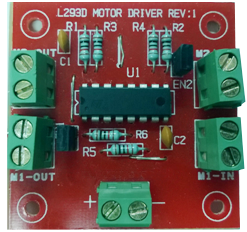
\includegraphics[width=\lgfig]{\LocDCMfig/dcmotor_board.png}
\caption{L293D motor driver board}
\label{fig:motordriverboard}
\end{figure}

Input from \arduino\ to H-bridge IC is in \index{pulse width
  modulation, PWM}%
pulse width modulation (PWM) form. PWM is a technique to generate
analog voltages using digital pins. We know that \arduino\ has digital
input-output pins. When these pins are configured as an output, they
provide High (5V) or Low (0V) voltage. With PWM technique, these pins
are switched on and off iteratively and fast enough so that the
voltage is averaged out to some analog value in between 0-5V. This
analog value depends on ''switch-on'' time and ''switch-off''
time. For example, if both ''switch-on'' time and ''switch-off'' time
are equal, average voltage on PWM pin will be 2.5V. To enable fast
switching of digital pin, a special hardware is provided in
microcontrollers.  PWM is considered as an important resource of
the microcontroller system. \arduino\ board has 6 PWM pins for each of
which, the input can come from 8 bits.  Thus we can generate 256
different analog values in between 0-5V with these pins.

We now carry out the following connections:
\begin{enumerate}
\item Connect input of L293D (M1\_IN) pins to two of the PWM pins
  available on \arduino.  We have used pins 9 and 10 of the \arduino\
  board. 
\item Connect the output of the L293D (M1\_OUT) pins directly to the 2
  wires of the DC motor.  As the direction is changed during the
  operation, the polarity of the connection does not matter.
\item Connect supply (Vcc) and ground (Gnd) pins of L293D to 5V and
  Gnd pins of the \arduino\ board, respectively.
\end{enumerate}
A schematic of these connections is given in
\figref{fig:dcm-schematic}.  The actual connections can be seen in
\figref{fig:dcmotorconn}.


\begin{figure}
\centering
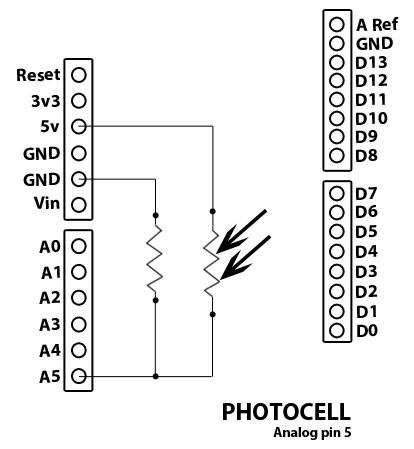
\includegraphics[width=\smfig]{\LocDCMfig/schematic.png}
\caption{A schematic of DC motor connections}
\label{fig:dcm-schematic}
\end{figure}
\begin{figure}
\centering
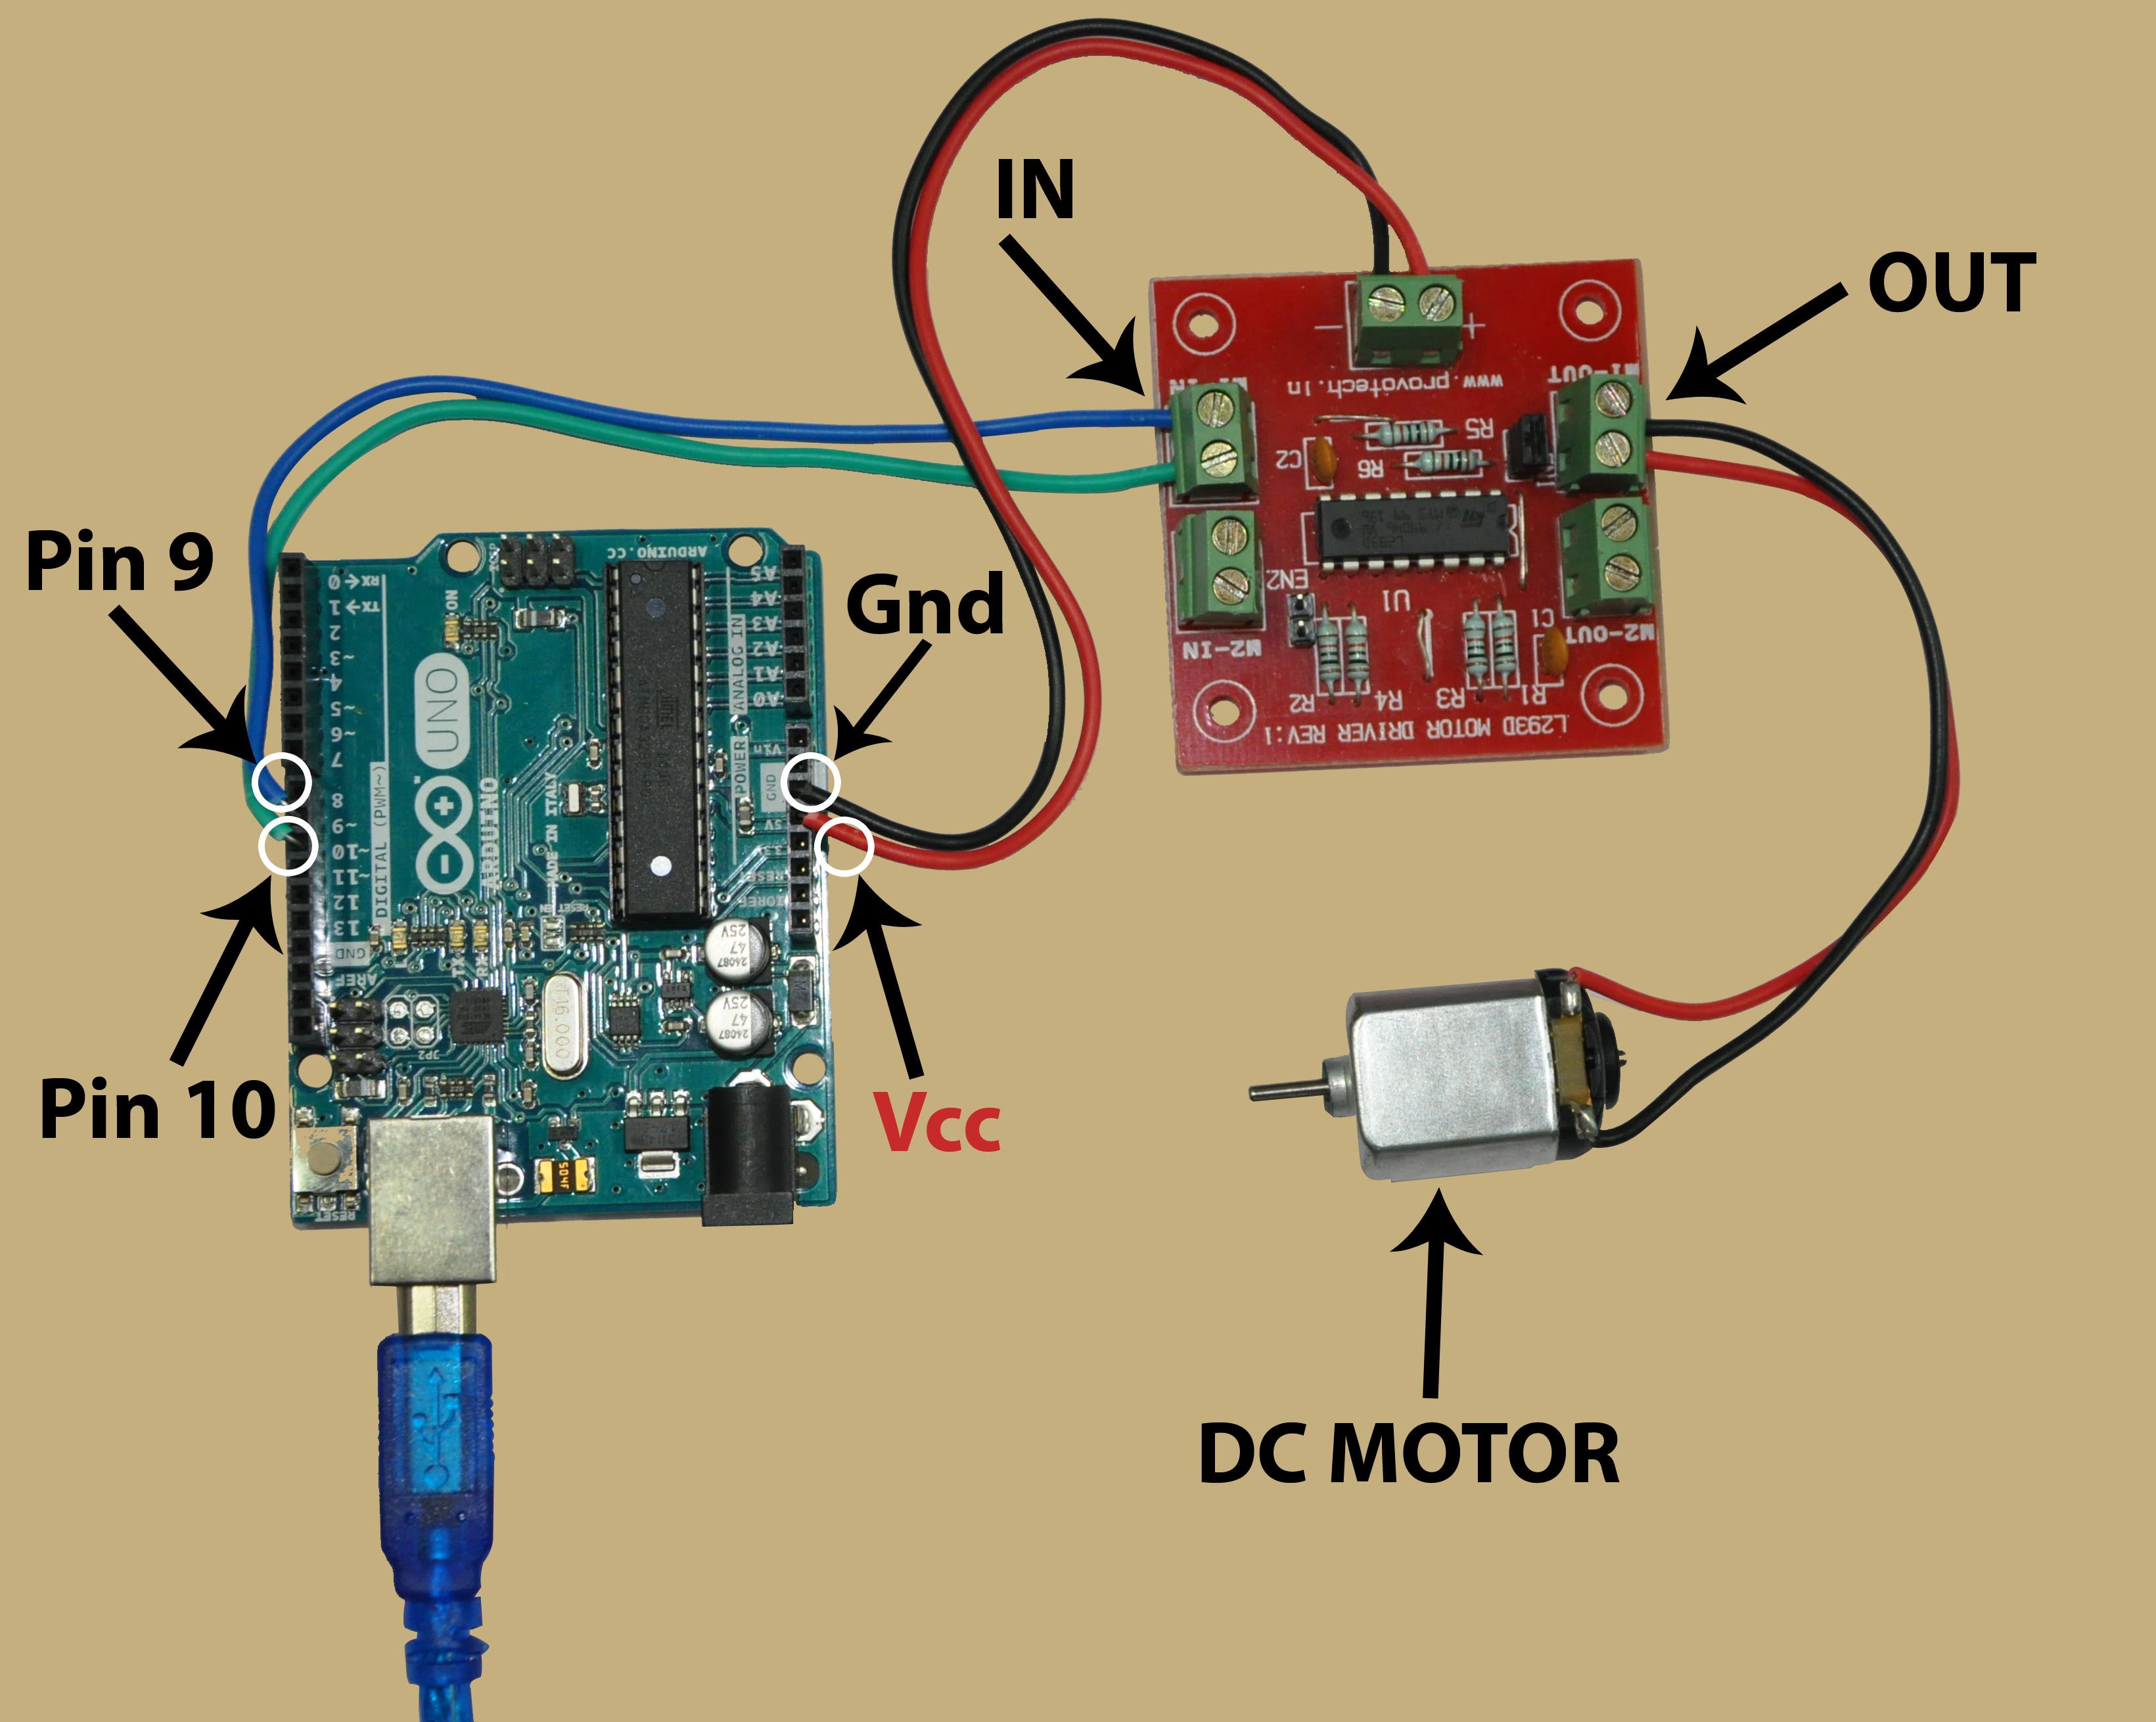
\includegraphics[width=\lgfig]{\LocDCMfig/dc_motor_description.jpg}
\caption{How to connect the DC motor to the \arduino\ board}
\label{fig:dcmotorconn}
\end{figure}

\section{Controlling the DC motor from Arduino}
\subsection{Controlling the DC motor}
\label{sec:dcm-ard}
In this section, we will describe some experiments that will help
drive the DC motor from the Arduino IDE.  We will also give the
necessary code.  We will present four experiments in this section.  We
assume the shield to be attached to the \arduino\ board while doing
these experiments.  The reader should go through the instructions
given in \secref{sec:ard-start} before getting started.
\begin{enumerate}
\item We now demonstrate how to drive the DC motor from the Arduino
  IDE.  \ardref{ard:dcmotor-clock} has the required code for this.  It
  starts the serial port at a baud rate of 9600.  Pins 9 and 10 are
  declared as output pins and hence values can be written on to them.
  Next, we write PWM 100 on pin 9 and PWM 0 on pin 10.  Recall from
  \figref{fig:dcmotorconn} that pins 9 and 10 are connected to the
  input of the breakout board, which in turn makes the DC motor run at
  an intermediate speed.  Recall from \secref{sec:led-pril} that a
  high on pin 9 also makes the blue LED come on.  As a result, the
  blue LED also lights up.

  Some of the breakout boards may not have enough current driving
  capability and hence tend to heat up.  To avoid these difficulties,
  the DC motor is run at an intermediate value of PWM 100.

  The line containing {\tt delay} makes the previous command execute
  for 3 seconds.  As a result, the DC motor continues to rotate for 3
  seconds.  After this, as we put a 0 in both pins 9 and 10, the motor
  comes to a halt.  The blue LED is also turned off.

\item It is easy to make the DC motor run in the reverse direction by
  interchanging the values put on pins 9 and 10.  This is done in
  \ardref{ard:dcmotor-both}.  In this program, we make the DC motor
  run in one direction for 3 seconds and then make it rotate in the
  reverse direction for 2 seconds.  The rotation in reverse direction
  is achieved by putting 100 in pin 10.  This makes the green LED
  light up, recall the discussion in \secref{sec:led-pril}.  After
  that, we release the motor by writing 0 in both pins 9 and 10.  This
  turns the green LED off.

\item Next, we make the DC motor run in forward and reverse
  directions, in a loop.  This is done through
  \ardref{ard:dcmotor-loop}.  We first put PWM 100 in the motor for 3
  seconds.  After that, make the motor stop for 2 seconds.  Finally,
  make the motor rotate in the reverse direction by putting PWM -100
  for two seconds.  Finally, we make the motor stop for one second.
  The entire thing is put in a loop.
\end{enumerate}

\begin{exercise}
Carry out the following exercise:
\begin{enumerate}
\item Try out some of the suggestions given above, \ie\ removing
  certain numbers from the code
\item See if the DC motor runs if you put 1 instead of 100 as the PWM
  value.  Explain why it does not run.  Find out the smallest value at
  which it will start running.
\end{enumerate}
\end{exercise}

\subsection{Arduino Code}
\label{sec:dcmotor-arduino-code}
\lstset{style=mystyle}
\addtocontents{ard}{\protect\addvspace{\codclr}}

\begin{ardcode}
\acaption{Rotating the DC motor}
{Rotating the DC motor.  Available at
  \LocDCMardbrief{dcmotor-clock/dcmotor-clock.ino}.}
\label{ard:dcmotor-clock}
\lstinputlisting{\LocDCMardcode/dcmotor-clock/dcmotor-clock.ino}
\end{ardcode}

\begin{ardcode}
\acaption{Rotating the DC motor in both directions}{Rotating the DC
  motor in both directions.  
  Available at
  \LocDCMardbrief{dcmotor-both/dcmotor-both.ino}.}
\label{ard:dcmotor-both}
\lstinputlisting{\LocDCMardcode/dcmotor-both/dcmotor-both.ino}
\end{ardcode}

\begin{ardcode}
\acaption{Rotating the DC motor in both directions in a loop}{Rotating
  the DC motor in both directions in a loop.
  Available at
  \LocDCMardbrief{dcmotor-loop/dcmotor-loop.ino}.}
\label{ard:dcmotor-loop}
\lstinputlisting{\LocDCMardcode/dcmotor-loop/dcmotor-loop.ino}
\end{ardcode}




\section{Controlling the DC motor from Scilab}
\label{sec:dcm-sci}
In this section, we will explain a few experiments to rotate the DC
motor.  We will first initialize it and then rotate it clockwise and
counterclockwise.  We will explain some of the other required
commands, such as sleep.

\subsection{Initialization}
In all the experiments in this section, we need to initialize the DC
motor first, using a \scilab\ command of the following type:

\begin{lstlisting}[style=nonumbers]
  cmd_dcmotor_setup(1,H-Bridge type,Motor number,PWM pin 1,PWM pin 2)
\end{lstlisting}
As mentioned earlier, number 1 in the above list refers to the
\arduino\ board.  We now discuss how to choose values for the other
parameters in this command.  As mentioned above, there are many
H-bridge IC manufacturers.  The inbuilt function {\tt
  cmd\_dcmotor\_setup} can work with most of the widely used ICs,
through a suitable input parameter.  Users have to provide the type
number of the breakout board they have.  Popular numbering convention
for different types of DC motor breakout boards is given in
\tabref{table:convention}.  For example, L293D is type 3.  Next, we
have to provide the motor number we want to control.  In our case, it
is number 1.  Finally we want to provide PWM pin numbers on \arduino.
As mentioned earlier, we are using pins 10 and 11.  In
\tabref{tab:dcmotor-init}, we list the choices that we have made.
Inserting these parameter values in the above shown \scilab\ command,
we get the following command \\
\lstinputlisting[firstline=2,lastline=2]
{\LocDCMscicode/dcmotor-clock.sce}
which is line number 2 in \sciref{sci:dcmotor-clock}.  We have already
seen 
the first two lines of this code and hence will not explain here.  We
will add more lines to this code as we go along.

\begin{table}
\centering
\caption{A numbering convention used in the DC motor breakout board}
\label{table:convention}
\begin{tabular}{|c|c|}\hline
DC Motor Type & Number \\ \hline
MotorShield Rev3 & 1 \\
PMODHB5/L298 & 2 \\
L293D & 3 \\ \hline
\end{tabular}
\end{table}
\begin{table}
\centering
\caption{Parameters for DC motor initialization}
\label{tab:dcmotor-init}
\begin{tabular}{|l|c|} \hline
Parameter & Value \\ \hline
H-Bridge type & 3 \\ 
Motor number & 1 \\
PWM 1 pin & 9 \\
PWM 2 pin & 10 \\ \hline
\end{tabular}
\end{table}

\subsection{Rotation for a specified time}
\label{sec:dc-both}
We will now explain how to run the DC motor.  We have to provide motor
number and the PWM value.  The \scilab\ command is of the form,
\begin{lstlisting}[style=nonumbers]
  cmd_dcmotor_run(1,Motor number,(sign)(PWM value))
\end{lstlisting}
Motor number is 1, as mentioned earlier.  Considering that the input
to a PWM pin comes from two 8 digital pins, we can provide values
between $-255$ and +255. Positive values correspond to clockwise
rotation while negative values correspond to anti-clockwise rotation.
Based on the PWM value and polarity, corresponding analog voltage is
generated.  We put a PWM value of 100 to make the DC motor to
run at an intermediate speed.  Assigning these values, we get the
following command:
\lstinputlisting[firstline=3,lastline=3]{\LocDCMscicode/dcmotor-clock.sce}
This is line number 3 in \sciref{sci:dcmotor-clock}.  This command
does not say for how long the motor should run.  This is taken care of
by the {\tt sleep} statement.  The units of sleep are milliseconds.
For example, line number 4 of \sciref{sci:dcmotor-clock}, given next,
says that \scilab\ should go to sleep for three seconds.
\lstinputlisting[firstline=4,lastline=4]{\LocDCMscicode/dcmotor-clock.sce}

Line number 5 of \sciref{sci:dcmotor-clock}, shown below, is mandatory
for every program.
\lstinputlisting[firstline=5,lastline=5]{\LocDCMscicode/dcmotor-clock.sce}
It releases the DC motor.  The PWM functionality on the \arduino\ pins
is ceased using this command.  This has the motor number as an input
parameter.

If the sleep command discussed above were not present, the DC motor
will not even run: soon after putting the value 100, the DC motor
would be released, leaving no time in between.  If on the other hand,
the DC motor is not released (\ie\ line number 6 being absent), the DC
motor will go on rotating.  Line number 6 of \sciref{sci:dcmotor-clock}
closes the serial port.

We encourage you to run the above code without either line numbers 4,
5 or 6 or all combinations.  Go ahead and do it - you will not break
anything.  At the most, you may have to unplug the USB cable and
restart the whole thing from the beginning.

\sciref{sci:dcmotor-clock} can easily be extended to make the DC motor
run in both directions.  The modified code is available in
\sciref{sci:dcmotor-both}.

\begin{exercise}
Carry out the following exercise:
\begin{enumerate}
\item Try out some of the suggestions given above, \ie\ removing
  certain numbers from the code
\item See if the DC motor runs if you put 1 instead of 100 as the PWM
  value.  Explain why it does not run.  Find out the smallest value at
  which it will start running.
\end{enumerate}
\end{exercise}

\subsection{Using the capabilities of \scilab}
Given that Scilab has a powerful programming syntax, a lot of
different experiments can be tried out.  We illustrate a few in this
section.  We begin with a {\tt for loop}.

In the previous section, we presented \sciref{sci:dcmotor-both}, where
we made the motor run in both directions, five seconds in the
clockwise direction and two seconds in reverse.  This code can be
embedded in a loop and the motor be made to repeat a certain number of
times.  This idea is implemented through \sciref{sci:dcmotor-loop}.
Through the {\tt for loop} in between line numbers 3 and 8, we make
the DC motor repeat four times the cycle containing one rotation in
each direction. 
%  \figref{fig:dcmotorfc} explains the entire operation
% through a flowchart.
% \begin{figure}
% \centering
% 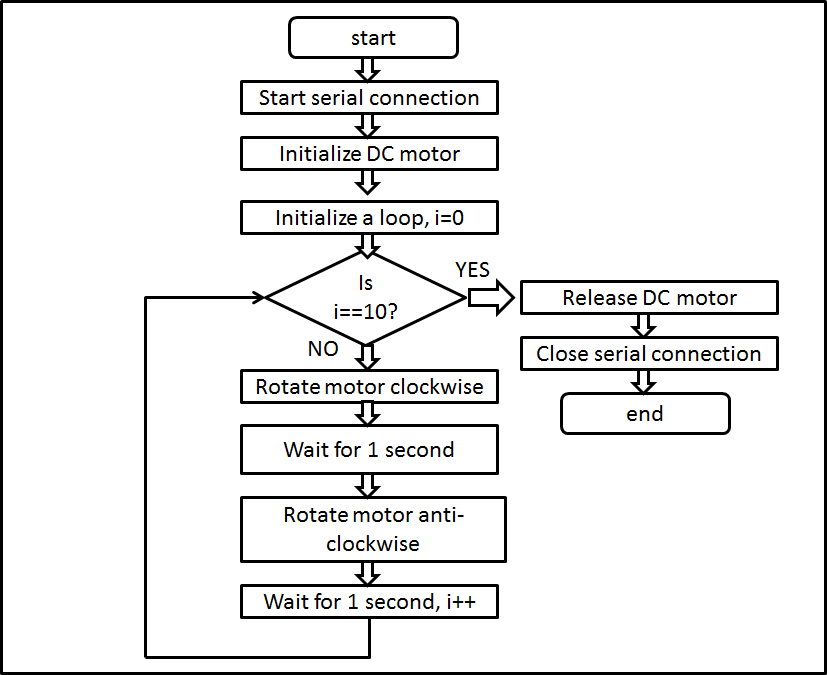
\includegraphics[width=\lgfig]{\LocDCMfig/dcmotorflowchart.png}
% \caption{Flowchart}
% \label{fig:dcmotorfc}
% \end{figure}

It is not difficult to see how some of the other features of the
\scilab\ programming language can be used along with this DC motor.
For example, it is possible to read a temperature value and based on
its value, start or stop the motor.  For real world applications, one
has to provide extra current carrying capabilities through external
hardware.  

\subsection{Scilab Code}
\label{sec:dcmotor-scilab-code}
\addtocontents{cod}{\protect\addvspace{\codclr}}

\begin{scicode}
\ccaption{Rotating the DC motor}
{Rotating the DC motor.  Available at
  \LocDCMscibrief{dcmotor-clock.sce}.}
\label{sci:dcmotor-clock}
\lstinputlisting{\LocDCMscicode/dcmotor-clock.sce}
\end{scicode}

\begin{scicode}
\ccaption{Rotating the DC motor in both directions}
{Rotating DC motor in both directions.  Available at
  \LocDCMscibrief{dcmotor-both.sce}.}
\label{sci:dcmotor-both}
\lstinputlisting{\LocDCMscicode/dcmotor-both.sce}
\end{scicode}

\begin{scicode}
\ccaption{Rotating the DC motor in both directions in a loop}{Rotating
  the DC motor in both directions in a loop.
  Available at
  \LocDCMscibrief{dcmotor-loop.sce}.}
\label{sci:dcmotor-loop}
\lstinputlisting{\LocDCMscicode/dcmotor-loop.sce}
\end{scicode}

\section{Controlling the DC Motor from Xcos}
In this section, we will see how to drive the DC motor from Xcos.  For
each experiment, we will give the location of the zcos file and the
parameters to set.  The reader should go through the instructions
given in \secref{sec:xcos-start} before getting started.  If the
rotation of the DC motor is blocked by any obstacle in any of the
experiments given below, you may want to hold it in your hand and let
it run unhindered.

\begin{enumerate}
\item First we will see a simple code that drives the DC motor for a
  specified time.  When the file required for this experiment is
  invoked, one gets the GUI as in \figref{fig:dcmotor-clock}.  In
  the caption of this figure, one can see where to locate the file.

  \begin{figure}
    \centering
    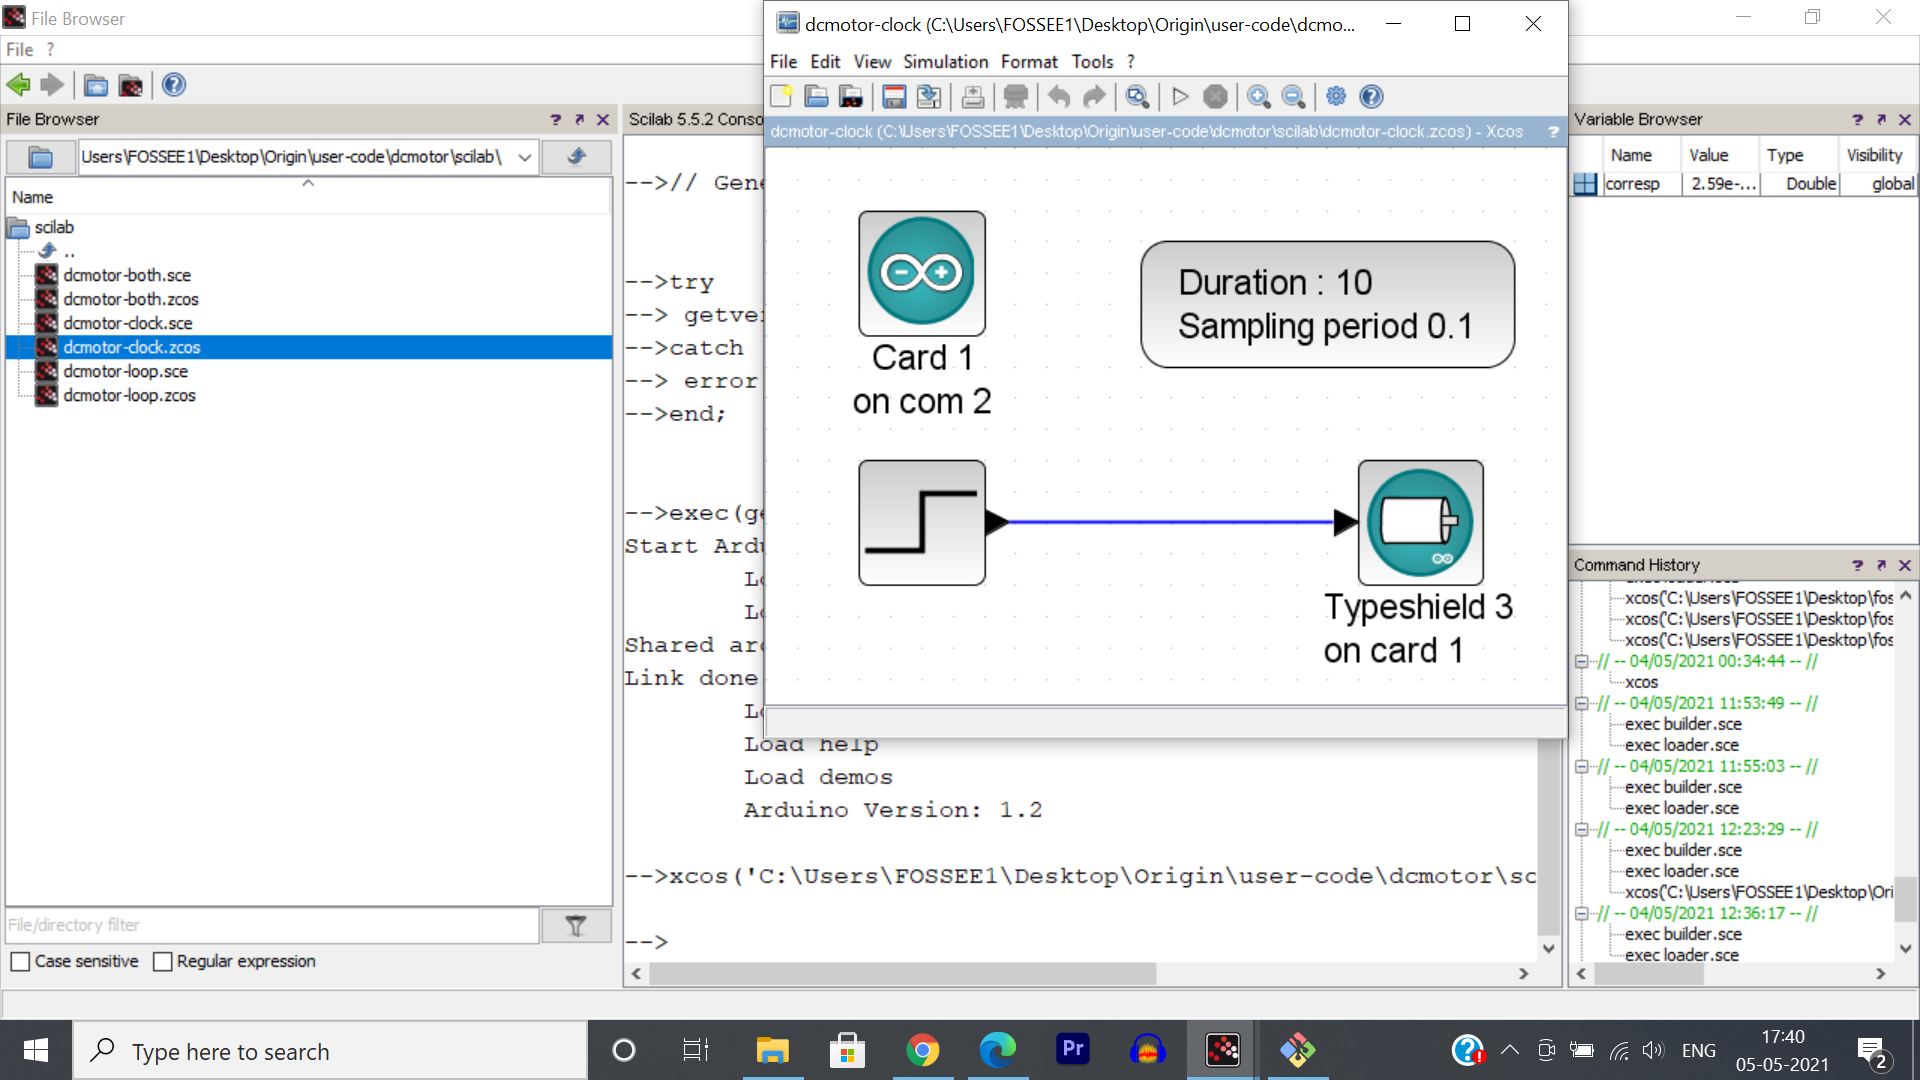
\includegraphics[width=\smfig]{\LocDCMfig/dcmotor-clock.png}
    \caption[Control of DC motor for a specified time from Xcos]
    {Control of DC motor for a specified time from Xcos.  This is what
      one sees when \LocDCMscibrief{dcmotor-clock.zcos}, is
      invoked.}
    \label{fig:dcmotor-clock}
  \end{figure}

  We will next explain how to set the parameters for this simulation.
  To set value on any block, one needs to right click and open the
  {\tt Block Parameters} or double click.  The values for each block
  is tabulated in \tabref{tab:dcmotor-clock}.  In case of {\tt
    DCMOTOR\_SB}, enter 3 to indicate for L293D board.  After clicking
  on OK, another box will pop up.  In that, enter the PWM pin numbers
  as 9 and 10 and click OK.  
All other parameters are to be left
  unchanged.
  \begin{table}
    \centering
    \caption{Xcos parameters to drive the DC motor for a specified time}
    \label{tab:dcmotor-clock}
    \begin{tabular}{llc} \hline
      Name of the block & Parameter name & Value \\ \hline
      ARDUINO\_SETUP & Identifier of Arduino Card & 1 \\
      & Serial com port number & 2\portcmd \\ \hline
      TIME\_SAMPLE & Duration of acquisition(s) & 10 \\
      & Sampling period(s) & 0.1 \\ \hline
      DCMOTOR\_SB & Type of Shield & 3 \\
      & Arduino card number & 1 \\ 
      & PWM pin numbers & 9 10 \\ 
      & Motor number & 1 \\ \hline
      STEP\_FUNCTION & Step time & 5 \\
      & Initial Value & 100 \\
      & Final Value & 0 \\ \hline
    \end{tabular}
  \end{table}

% Can you find out for how long the DC motor will run when this program
% is executed?  In which block do we provide this information?  The
% answer is that the DC motor will stop only when we terminate the
% program.  As in the previous experiments, we can terminate the Xcos
% program by pressing the stop button.  The DC motor gets released when
% the stop button is pressed.



\item Next, we will describe the Xcos code that drives the DC motor in
  both forward and reverse directions.  When the file required for
  this experiment is invoked, one gets the GUI as in
  \figref{fig:dcmotor-both}.  In the caption of this figure, one can
  see where to locate the file.

  \begin{figure}
    \centering
    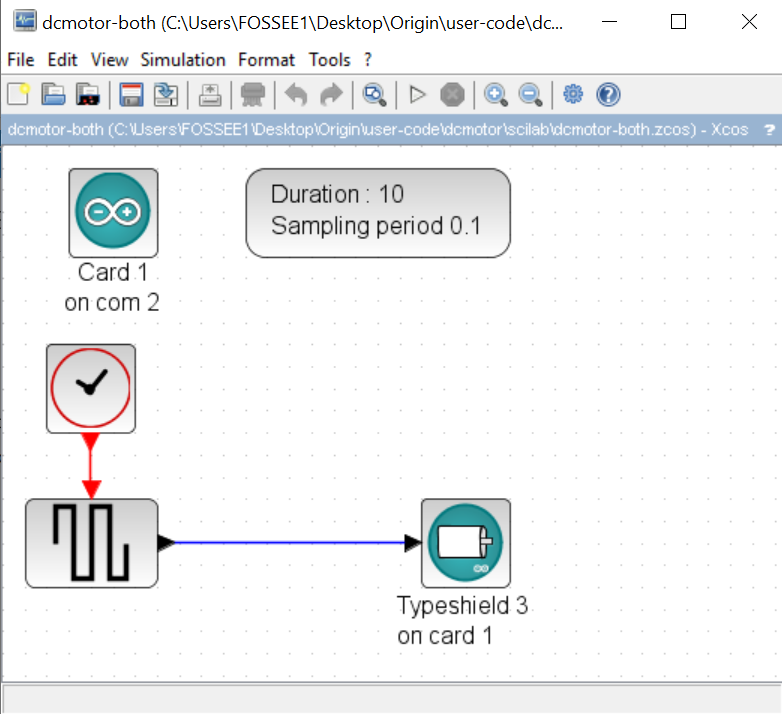
\includegraphics[width=\smfig]{\LocDCMfig/dcmotor-both.png}
    \caption[Xcos control of the DC motor in forward and reverse
    directions]{Xcos control of the DC motor in forward and reverse
      directions.  This is what one sees when
        \LocDCMscibrief{dcmotor-both.zcos}, is invoked.}
    \label{fig:dcmotor-both}
  \end{figure}

  We will next explain how to set the parameters for this simulation.
  To set value on any block, one needs to right click and open the
  {\tt Block Parameters} or double click.  The values for each block
  is tabulated in \tabref{tab:dcmotor-both}.  All other parameters are
  to be left unchanged.
  \begin{table}
    \centering
    \caption{Xcos parameters to drive the DC motor in forward and
      reverse directions}
    \label{tab:dcmotor-both}
    \begin{tabular}{llc} \hline
      Name of the block & Parameter name & Value \\ \hline
      ARDUINO\_SETUP & Identifier of Arduino Card & 1 \\
      & Serial com port number & 2\portcmd \\ \hline
      TIME\_SAMPLE & Duration of acquisition(s) & 10 \\
      & Sampling period(s) & 0.1 \\ \hline
      DCMOTOR\_SB & Type of Shield & 3 \\
      & Arduino card number & 1 \\ 
      & PWM pin numbers & 9 10 \\ 
      & Motor number & 1 \\ \hline
      STEP\_FUNCTION & Step time & 5 \\
      & Initial Value & 100 \\
      & final value & 0 \\ \hline
      CLOCK\_c & Period & 1 \\
      & Initialisation Time & 0.1 \\ \hline
    \end{tabular}
  \end{table}

\item Next, we will describe the Xcos code that drives the DC motor in
  a loop.  When the file required for
  this experiment is invoked, one gets the GUI as in
  \figref{fig:dcmotor-loop}.  In the caption of this figure, one can
  see where to locate the file.

  \begin{figure}
    \centering
    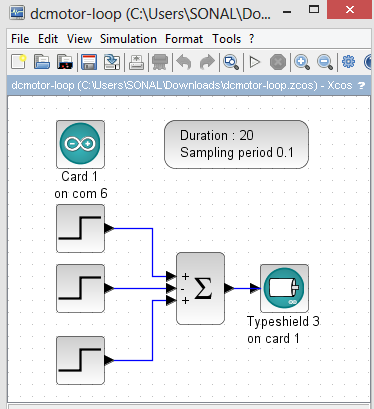
\includegraphics[width=\smfig]{\LocDCMfig/dcmotor-loop.png}
    \caption[Xcos control of the DC motor in forward and reverse
    directions]{Xcos control of the DC motor in forward and reverse
      directions.  This is what one sees when
        \LocDCMscibrief{dcmotor-loop.zcos}, is invoked.}
    \label{fig:dcmotor-loop}
  \end{figure}

  We will next explain how to set the parameters for this simulation.
  To set value on any block, one needs to right click and open the
  {\tt Block Parameters} or double click.  The values for each block
  is tabulated in \tabref{tab:dcmotor-loop}.  All other parameters are
  to be left unchanged.
  \begin{table}
    \centering
    \caption{Xcos parameters to drive the DC motor in a loop}
    \label{tab:dcmotor-loop}
    \begin{tabular}{llc} \hline
      Name of the block & Parameter name & Value \\ \hline
      ARDUINO\_SETUP & Identifier of Arduino Card & 1 \\
      & Serial com port number & 2\portcmd \\ \hline
      TIME\_SAMPLE & Duration of acquisition(s) & 10 \\
      & Sampling period(s) & 0.1 \\ \hline
      DCMOTOR\_SB & Type of Shield & 3 \\
      & Arduino card number & 1 \\
      & PWM pin numbers & 9 10 \\ 
      & Motor number & 1 \\ \hline
      STEP\_FUNCTION 1 & Step time & 3 \\
      & Initial Value & 100 \\
      & Final Value & 0 \\ \hline
      STEP\_FUNCTION 2 & Step time & 5 \\
      & Initial Value & 0 \\
      & Final Value & 100 \\ \hline
      STEP\_FUNCTION 3 & Step time & 7 \\
      & Initial Value & 0 \\
      & Final Value & 100 \\ \hline
      BIGSOM\_f & Inputs ports signs/gain & [1;-1;1] \\ \hline
    \end{tabular}
  \end{table}
\end{enumerate}


%\section{Do we need any of these? \redcolor{Manas, please answer}}
%   \begin{figure}
%     \centering
%     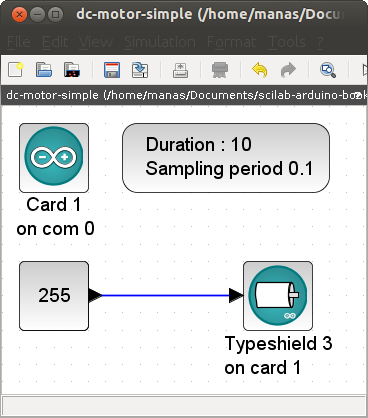
\includegraphics[width=\smfig]{\LocDCMfig/dc-motor-simple.png}
%     \caption[Control of DC motor from Xcos]{Control of DC motor from
%       Xcos.  This is what one sees when {\tt
%         \LocDCMscibrief/dc-motor-simple.zcos} is invoked.}
%     \label{fig:dcm-xcos-simple}
%   \end{figure}



% \begin{enumerate}
% \item Card 1 on com 5 block: Right-click and open the block properties
%   or double click on this block.  In the resulting dialog window,
%   enter the com port number of your system.
% \item Typeshield 1 on card 1: Following the procedure mentioned above,
%   make sure that the entry for this block is 3, which corresponds to
%   L293D breakout board, as explained in \tabref{table:convention}. 
% \end{enumerate}
% Leave the other blocks unchanged.

% This Xcos program is used to put a specific PWM value to the DC motor.
% We can right click (or double click) on any block and see what
% parameter values are present in it.  By doing this, we can see that
% this program is used to put in a PWM value of 255.  Start executing
% the program by pressing the right arrow key.  

\begin{exercise} 
Carry out the following exercise:
\begin{enumerate}
\item Keep reducing the PWM value and find out the minimum value
  required to run the DC motor.  Is this value in agreement with what
  we found in the previous section?
\item Change the PWM value to $-100$ and check if the DC motor rotates
  in the opposite direction.
\item Find out the smallest PWM value required to make the motor run
  in the opposite direction.  That is, find the least count for both
  directions.
\item Come up with a method to rotate the motor in two directions for
  different time periods.
\end{enumerate}
\end{exercise}

\section{Controlling the DC Motor from Python}
\subsection{Controlling the DC Motor}
In this section, we will explain a few experiments to rotate the DC
motor. We will first initialize it and then rotate it clockwise and
counterclockwise. We will explain some of the other required commands,
such as sleep.

Initialization: In all the experiments in this section, we need to
initialize the DC motor first, using a Python command of the following
type:
\begin{lstlisting}[style=nonumbers]
  cmd_dcmotor_setup(1,H-Bridge type,Motor number,PWM pin 1,PWM pin 2)
\end{lstlisting}

As mentioned earlier, number 1 in the above list refers to the Arduino Uno board.
We now discuss how to choose values for the other parameters in this command. As
mentioned above, Popular numbering convention for different types of DC motor breakout
boards is given in Table 7.1. For example, L293D is type 3. Next, we have to provide
the motor number we want to control. In our case, it is number 1. Finally we want
to provide PWM pin numbers on Arduino Uno. As mentioned earlier, we are using
pins 10 and 11. In Table 7.2, we list the choices that we have made. Inserting these
parameter values in the above shown Python command, we get the following command

self.obj\_arduino.cmd\_dcmotor\_setup(1,3,1,self.pin1,self.pin2)

To rotate the motor,we have to provide motor number
and the PWM value. The Python command is of the form,

cmd\_dcmotor\_run ( 1 , Motor number , ( sign ) (PWM value ) )

The PWM values to be given are as same as explained in Scilab code before.

To run the motor for specified amount of time,we will use sleep command

sleep(3) //sleep for 3 seconds

To release the dc motor, we will use the following command

cmd\_dcmotor\_release(1,1) //Motor 1 is release

To run motor in loop, for loop is used in Python code 7.3.

\subsection{Python Code}
\label{sec:dcmotor-python-code}
\addtocontents{pyd}{\protect\addvspace{\codclr}}

\begin{pycode}
\pcaption{Rotating the DC motor}
{Rotating the DC motor.  Available at
  \LocDCMpybrief{dcmotor-clock.py}.}
\label{py:dcmotor-clock}
\lstinputlisting{\LocDCMpycode/dcmotor-clock.py}
\end{pycode}

\begin{pycode}
\pcaption{Rotating the DC motor in both directions}
{Rotating DC motor in both directions.  Available at
  \LocDCMpybrief{dcmotor-both.py}.}
\label{py:dcmotor-both}
\lstinputlisting{\LocDCMpycode/dcmotor-both.py}
\end{pycode}

\begin{pycode}
\pcaption{Rotating the DC motor in both directions in a loop}{Rotating
  the DC motor in both directions in a loop.
  Available at
  \LocDCMpybrief{dcmotor-loop.py}.}
\label{py:dcmotor-loop}
\lstinputlisting{\LocDCMpycode/dcmotor-loop.py}
\end{pycode}

\section{Controlling the DC Motor from Julia}
\subsection{Controlling the DC Motor}

In this section, we will explain a few experiments to rotate the DC
motor. We will first initialize it and then rotate it clockwise and
counterclockwise. We will explain some of the other required commands,
such as sleep.

Initialization: In all the experiments in this section, we need to
initialize the DC motor first, using a Julia command of the following
type:
\begin{lstlisting}[style=nonumbers]
  DCMotorSetup(1,H-Bridge type,Motor number,PWM pin 1,PWM pin 2)
\end{lstlisting}


We now discuss how to choose values for the other parameters in this
command. As mentioned above, choose the H-bridge accordingly as
explained previously. THis is the second parameter given to the
DCMotorSetup function. Next, we have to provide the motor number we
want to control. In our case, it is number 1. Finally we want to
provide PWM pin numbers on Arduino Uno. As mentioned earlier, we are
using pins 9 and 10. In Table 7.2, we list the choices that we have
made. Inserting these parameter values in the above shown Julia
function command, we get the following command

DCMotorSetup(1,3,1,9,10)

To rotate the motor,we have to provide motor number
and the PWM value. The Julia command is of the form,

DCMotorRun ( 1 , Motor number , ( sign ) (PWM value ) )

The PWM values to be given are as same as explained in Scilab code before.

To run the motor for specified amount of time,we will use the sleep command

sleep(3) //sleep for 3 seconds

To release the dc motor, we will use the following command

DCMotorRelease(ser,1) //Motor 1 is release

To run motor in loop, for loop is used in Julia code 7.3.

\subsection{Julia Code}
\label{sec:dcmotor-julia-code}
\addtocontents{juliad}{\protect\addvspace{\codclr}}

\begin{juliacode}
\jcaption{Rotating the DC motor}
{Rotating the DC motor.  Available at
  \LocDCMjuliabrief{dcmotor-clock.jl}.}
\label{julia:dcmotor-clock}
\lstinputlisting{\LocDCMjuliacode/dcmotor-clock.jl}
\end{juliacode}

\begin{juliacode}
\jcaption{Rotating the DC motor in both directions}
{Rotating DC motor in both directions.  Available at
  \LocDCMjuliabrief{dcmotor-both.jl}.}
\label{julia:dcmotor-both}
\lstinputlisting{\LocDCMjuliacode/dcmotor-both.jl}
\end{juliacode}

\begin{juliacode}
\jcaption{Rotating the DC motor in both directions in a loop}{Rotating
  the DC motor in both directions in a loop.
  Available at
  \LocDCMjuliabrief{dcmotor-loop.jl}.}
\label{julia:dcmotor-loop}
\lstinputlisting{\LocDCMjuliacode/dcmotor-loop.jl}
\end{juliacode}


\section{Controlling the DC Motor from OpenModelica}
\subsection{Controlling the DC Motor}
Initialization of DC Motor : In all the experiments in this section,
we need to initialize the DC motor first, using a OpenModelica command
of the following type:

\begin{lstlisting}[style=nonumbers]
  cmd_dcmotor_setup(1,H-Bridge type,Motor number,PWM pin 1,PWM pin 2)
\end{lstlisting}
cmd\_dcmotor\_setup(1,3,1,9,10)

To rotate the motor,we have to provide motor number
and the PWM value. The OpenModelica command is of the form,

cmd\_dcmotor\_run ( 1 , Motor number , ( sign ) (PWM value ) )

The PWM values to be given are as same as explained in Scilab code before.

To run the motor for specified amount of time,we will use sleep command

delay(2000) //sleep for 2 seconds

To release the dc motor, we will use the following command

cmd\_dcmotor\_release(ser,1) //Motor 1 is release

To run motor in loop, for loop is used in OpenModelica code 7.3

%%%%%%%OpenModelica description ends

% \subsection{Using the Xcos features in DC motor control}
% Xcos can be used to control the DC motor in many different ways.  In
% this section, we will see a few approaches.  First, we will make the
% DC motor start and stop.  For this, we will open the program given in \figref{fig:dcm-xcos-start-stop}.
% \begin{figure}
% \centering
% 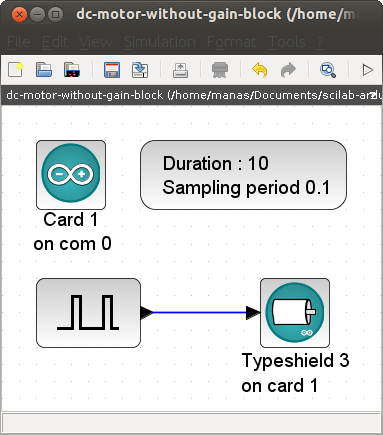
\includegraphics[width=\smfig]{\LocDCMfig/dc-motor-start-stop.png}
% \caption[Xcos program to make the DC motor to rotate, pause and
%   repeat]{Xcos program to make the DC motor to rotate, pause and
%   repeat.  This is what one sees when {\tt
%     \LocDCMscibrief/dc-motor-start-stop.zcos} is invoked.}
% \label{fig:dcm-xcos-start-stop}
% \end{figure}

% The input is a train of pulses of positive values.  The amplitude of
% these pulses is chosen to be 255.  The period is chosen to be 1s.
% \redcolor{these values have to be checked - this section to be
%   rewritten.}  On executing this Xcos code, the DC motor rotates for
% 1s, pauses for 1s, and repeats.  This continues until the Xcos program
% is terminated.

% \begin{exercise}
% Carry out the following exercise:
% \begin{enumerate}
% \item The user may repeat this exercise with different amplitude and
%   periods. 
% \item The above may be repeated with negative PWM values.
% \item One may find the least count for all experiments.
% \end{enumerate}
% \end{exercise}

% We will next see how to give positive and negative values of PWM in
% the same experiment.  For this, we will use the Xcos program given in
% \figref{fig:dcm-xcos-both}.  This code is similar to the previous one,
% but for a few minor changes.  First of all, we have introduced a gain
% block, and assigned a value of 255.  This block is excited by pulses
% of $+1$ and $-1$ alternately.  This simple approach, however, results
% in the DC motor running in both directions for identical durations.
% \begin{figure}
% \centering
% 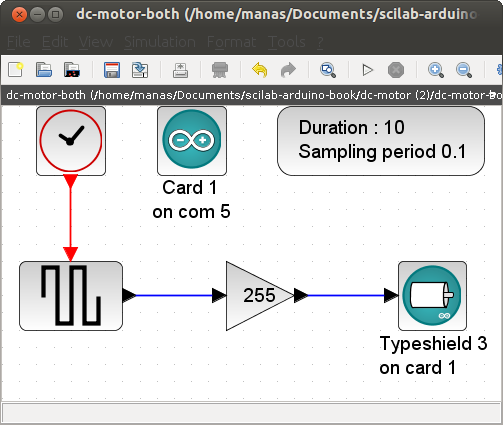
\includegraphics[width=\lgfig]{\LocDCMfig/dc-motor-both.png}
% \caption[Xcos program to make the DC motor to rotate, pause and to
%   rotate in the opposite direction]{Xcos program to make the DC motor
%   to rotate, pause and to rotate in the opposite direction.  This is
%   what one sees when {\tt \LocDCMscibrief/dc-motor-both.zcos} is
%   invoked.}
% \label{fig:dcm-xcos-both}
% \end{figure}

% \begin{exercise}
% Carry out the following exercise:
% \begin{enumerate}
% \item Repeat this experiment for different amplitudes and periods.
% \end{enumerate}
% \end{exercise}


% \subsection{Troubleshooting \redcolor{Do we need this? - Manas, please answer}}
% \begin{enumerate}
% \item If we want to connect external supply, Ground (Gnd) pin of L293D board, external supply and \arduino\ board should be shorted. This creates common ground voltage for entire set-up.
% \item We can connect more than one motor simultaneously using H-bridge like L293D. Typically break-out boards support 2 motors. However we are limited by number of PWM pins available on the board. For each motor cable of bidirectional motion, we need two PWM pins
% \end{enumerate}


\subsection{OpenModelica Code}
\label{sec:dcmotor-OpenModelica-code}
\addtocontents{OpenModelicad}{\protect\addvspace{\codclr}}

\begin{OpenModelicacode}
\mcaption{Rotating the DC motor}
{Rotating the DC motor.  Available at
  \LocDCMOpenModelicabrief{dcmotor-clock.mo}.}
\label{OpenModelica:dcmotor-clock}
\lstinputlisting{\LocDCMOpenModelicacode/dcmotor-clock.mo}
\end{OpenModelicacode}

\begin{OpenModelicacode}
\mcaption{Rotating the DC motor in both directions}
{Rotating DC motor in both directions.  Available at
  \LocDCMOpenModelicabrief{dcmotor-both.mo}.}
\label{OpenModelica:dcmotor-both}
\lstinputlisting{\LocDCMOpenModelicacode/dcmotor-both.mo}
\end{OpenModelicacode}

\begin{OpenModelicacode}
\mcaption{Rotating the DC motor in both directions in a loop}{Rotating
  the DC motor in both directions in a loop.
  Available at
  \LocDCMOpenModelicabrief{dcmotor-loop.mo}.}
\label{OpenModelica:dcmotor-loop}
\lstinputlisting{\LocDCMOpenModelicacode/dcmotor-loop.mo}
\end{OpenModelicacode}
%%%%%%%%%%OpenModelica code ends
